\documentclass[a4paper]{amsart}
\usepackage[utf8]{inputenc}
\usepackage{lmodern}
\usepackage{microtype}

\usepackage{commath}

\usepackage{tikz}
\usepackage{graphicx}

\usepackage[hidelinks]{hyperref}
\usepackage[noabbrev]{cleveref}

\def\signed #1{{\leavevmode\unskip\nobreak\hfil\penalty50\hskip2em
  \hbox{}\nobreak\hfil(#1)%
  \parfillskip=0pt \finalhyphendemerits=0 \endgraf}}
\newsavebox\mybox
\newenvironment{aquote}[1]
  {\savebox\mybox{#1}\begin{quote}}
  {\signed{\usebox\mybox}\end{quote}}

\swapnumbers
\newtheorem{thm}{Theorem}[section]
\newtheorem{lem}[thm]{Lemma}
\theoremstyle{definition}
\newtheorem{defn}[thm]{Definition}
\newtheorem{ex}[thm]{Example}
\newtheorem{exercise}[thm]{Exercise}
\theoremstyle{remark}
\newtheorem{rem}[thm]{Remark}


\title[Generic Skills in Maths]{A Journey Through Generic Skills\\for Level Three and Scholarship Calculus}
\author{Alex Elzenaar}
\date{\today}

\begin{document}
\maketitle
\tableofcontents
\section{Introduction}
This document introduces some of the basic skills for L3/Scholarship calculus that
do not fit nicely into any of the standards. The two big results that we obtain are
the Binomial Theorem (i.e. the general expansion of $ (x + y)^n $), and a solution
of the Seven Bridges of K\"onigsberg problem.

\section{Set Notation}
We begin by quoting from Paul Halmos' classic book, \textit{Naive Set Theory}.
\begin{aquote}{Halmos}
  A pack of wolves, a bunch of grapes, or a flock of pigeons are all examples of sets of things. The mathematical concept of a set can
  be used as the foundation for all known mathematics...
\end{aquote}
Like Halmos, we will avoid an exact definition of sets so that we do not need to deal with the logical issues that come
with it (does the set of all sets that do not contain themselves contain itself?) --- for us, a set is simply a collection
of objects.

The simplest way to write a set is to list its members (elements). We do need the following definition:
\begin{ex}\label{ex:set3}
  The set $ X = \{1, 2, 3\} $ has three members. The set $ X' = \{ 1, 2, 1, 1, 1, 2, 2, 3\} $ is \textbf{equal} to the set $ X $,
  since the two contain the same elements.
\end{ex}

\begin{defn}
  The \textbf{cardinality} of a finite set is the number of elements that it contains --- we write $ \abs{S} $ for the cardinality of some set $ S $.
\end{defn}

This definition is very naive and does not stand up to much thought (we want to be able to define numbers in terms of sets, so how does it
make sense to talk about the `number' of elements in a set?) --- so we will avoid thinking about it. Suffice it to say that there is a more
rigorous definition.

\begin{ex}
  $ \abs{X} = 3 $, where $ X $ is as given in \cref{ex:set3} above.
\end{ex}

\begin{defn}
  We define the following infinite sets intuitively:
  \begin{enumerate}
    \item The set $ \mathbb{N} $ is the set of \textbf{natural numbers}: $ 1, 2, 3, ... $
    \item The set $ \mathbb{Z} $ is the set of \textbf{integers}: $ ..., -2, -1, 0, 1, 2, ... $
    \item The set $ \mathbb{Q} $ is the set of \textbf{rational numbers}: all numbers of the form $ p/q $, where $ p $ and $ q \neq 0 $ are
          integers (and $ p $ and $ q $ share no factors).
    \item The set $ \mathbb{R} $ is the set of \textbf{real numbers}: the rational numbers together with the limit of every convergent
          sequence of rationals. Examples of irrational real numbers include $ \pi $, $ \sqrt{p} $ for any
          prime $ p $,\footnote{~See \cref{thm:irrational}} $ e $.
    \item The set $ \mathbb{P} $ is the set of \textbf{prime numbers}: natural numbers with exactly two factors.
    \item The set $ \mathbb{Z}^+ $ is the set of \textbf{non-negative} integers: the natural numbers together with zero.
  \end{enumerate}
\end{defn}

\begin{rem}
  We will not define `cardinality' or `size' for infinite sets. However, even though all the sets above are infinite (we will prove
  later that there are infinitely many primes), it is possible to show that the real numbers are in some sense greater in number
  than the natural numbers and integers; and that the sets of natural numbers, primes, integers, and rationals are all the same size.
\end{rem}

\begin{defn}
  The following symbols are a convenient shorthand:

  \begin{enumerate}
    \item We write $ x \in X $ if $ x $ is an element (member) of $ X $.
    \item We write $ S \subseteq X $ if every element of $ S $ is also an elemnt of $ X $.
  \end{enumerate}
\end{defn}

\begin{ex}
  $ \mathbb{P} \subseteq \mathbb{N} \subseteq \mathbb{Z}^+ \subseteq \mathbb{Z} \subseteq \mathbb{Q} \subseteq \mathbb{R} $.
\end{ex}

\begin{defn}[Axiom of Extension]
  Suppose $ X $ and $ Y $ are sets. If $ X \subseteq Y $ and $ Y \subseteq X $, then $ X = Y $.
\end{defn}

\begin{exercise}
  Convince yourself that the axiom of extension is equivalent to writing that ``$ X = Y $ if $ X $ and $ Y $ share the same elements''.
\end{exercise}

\begin{thm}
  There is a unique set with no elements.\footnote{~Note that we have not proved that there exists any set at all... this may seem
  self-evident, but it must be explicitly assumed in any rigorous set theory. We are not developing a rigorous set theory, so we will
  avoid the question entirely.}
\end{thm}
\begin{proof}
  Suppose that $ \abs{A} = \abs{B} = 0 $. Now, $ A \neq B $ if and only if there is some element in $ A $ that is not in $ B $,
  or some element in $ B $ that is not in $ A $. Plainly, there is no such element in either case; so the statement $ A \neq B $ is
  false and $ A = B $.
\end{proof}

\begin{rem}
  Since there is exactly one set with no elements (called the empty set), we assign it the symbol $ \emptyset $.
\end{rem}

\begin{exercise}
  Suppose $ X $ is a set. Show that $ \emptyset \subseteq X $ and $ X \subseteq X $.
\end{exercise}

Obviously for more complicated sets, listing the elements out is difficult.
\begin{ex}\label{ex:sumsquare}
  Let $ S $ be the set of all even integers that cannot be written as the sum of two exactly primes.
  It is thought that in fact it will be very simple to write out the list of elements of $ S $; in fact,
  it has been conjectured that $ S = \emptyset $. Hence, at the current time it is very difficult to
  list the elements of $ S $, as not only are their identities unknown but their existence is in doubt!
\end{ex}

We introduce `set-builder notation' to solve this problem.
\begin{defn}
  Let $ X $ be a set.  Let $ P(x) $ be a function that maps a value $ x \in X $ to a boolean value (i.e. true or false). Then
  the subset $ A \subseteq X $ which contains all those elements of $ x $ such that $ P(x) = T $ exists, and is denoted by
  $ A = \{ x \in X : P(x) \} $ (read $ A $ is the set of all elements $ x $ of $ X $ such that $ P(x) $).
\end{defn}

\begin{ex}
  The set $ S $ from \cref{ex:sumsquare} can be more formally written as $ S = \{ x \in 2\mathbb{Z}: x \neq p + q \text{ for any } p, q \in \mathbb{P}\} $.
\end{ex}

\begin{exercise}
  Show that the sets $ A = \{x \in \mathbb{Q} : x^2 + 5x + 6 = 0 \} $ and $ B = \{-2, -3\} $ are equal.
\end{exercise}

\begin{defn}
  Two important set operations are intersection ($ \cap $) and union ($ \cup $). Suppose that $ X $ and $ Y $ are both
  subsets of some set $ \mathcal{U} $. Then:
  \begin{enumerate}
    \item $ X \cap Y := \{x \in \mathcal{U} : x \in X \text{ and } x \in Y \}. $
    \item $ X \cup Y := \{x \in \mathcal{U} : x \in X \text{ or } x \in Y \text{ (or both)}\}. $
  \end{enumerate}
\end{defn}

\begin{ex}
  If $ X = \{1, 2, 3\} $ and $ Y = \{0, 2, 4\} $ then $ X \cap Y = \{2\} $ and $ X \cup Y = \{0, 1, 2, 3, 4\} $.
\end{ex}

\begin{exercise}
  If $ X $ is an arbitrary set, show that $ X \cap X = X \cup X = X \cup \emptyset = X $, and that $ X \cap \emptyset = \emptyset $.
\end{exercise}

\begin{exercise}
  If $ A = \{i,\allowbreak t,\allowbreak w,\allowbreak a,\allowbreak s,\allowbreak a,\allowbreak d,\allowbreak a,\allowbreak r,\allowbreak k,
  \allowbreak a,\allowbreak n,\allowbreak d\} $ and $ B = \{s,\allowbreak t,\allowbreak o,\allowbreak r,\allowbreak m,\allowbreak y,\allowbreak n,
  \allowbreak i,\allowbreak g,\allowbreak h,\allowbreak t\} $, find $ A \cap B $ and $ A \cup B $.
\end{exercise}

\section{Mathematical Proof}
What is a mathematical proof?
\begin{itemize}
  \item A proof is an explanation of why a statement is true. (Kevin Houston, \textit{How to Think Like a Mathematician})
  \item A proof is a logical argument in which the true premises provide conclusive reasons for the conclusion. (Pr$\infty$fWiki)
  \item A mathematical proof is a way to show that a mathematical theorem is true. One must show that the theorem is true in all cases. (Simple English Wikipedia)
\end{itemize}

An interesting essay on the subject is \textit{On Proof and Progress in Mathematics} by William Thurston.\footnote{~arXiv:math/9404236v1 [math.HO] 1 Apr 1994}

\begin{exercise}
  Suppose that $ A \implies B $, and $ B $ is false. What can you say about the truth value of $ A $? What if $ B $ is true?
\end{exercise}

\begin{exercise}
  Critique the argument:
  \begin{displaymath}
    2 = 4 \Rightarrow 2\pi = 4\pi \Rightarrow \sin 2\pi = \sin 2\pi \Rightarrow 0 = 0,
  \end{displaymath}
  so $ 2 = 4 $.
\end{exercise}

The proof of the following theorem is quite cute.

\begin{thm}
  There exist irrational numbers $ a $ and $ b $ such that $ a^b $ is rational.
\end{thm}
\begin{proof}
  Suppose that $ \sqrt{2}^{\sqrt{2}} $ is rational. Then we are done. Otherwise, $ \sqrt{2}^{\sqrt{2}} $ is irrational;
  consider $ (\sqrt{2}^{\sqrt{2}})^{\sqrt{2}} = \sqrt{2}^2 = 2 $ which is obviously rational.\footnote{~It has been proved
  that $ \sqrt{2}^{\sqrt{2}} $ is, in fact, irrational.}
\end{proof}

\begin{rem}
  In this section, we must take on faith the following facts:
  \begin{enumerate}
    \item In any subset of the natural numbers, there is a smallest element.
    \item If a prime divides a product of two numbers, then it divides (at least) one of the two numbers.
  \end{enumerate}
\end{rem}

\begin{exercise}
  Suppose that $ a \in \mathbb{Q} $ and $ a^2 \in \mathbb{Z} $. Prove that $ a \in \mathbb{Z} $. [\emph{Think about what it means for a number to be rational.}]
\end{exercise}

\begin{thm}\label{thm:irrational}
  The real number $ \sqrt{p} $ is irrational for all $ p \in \mathbb{P} $.
\end{thm}
\begin{proof}
  Suppose, in order to force a contradiction, that $ p = \left(\frac{m}{n}\right)^2 $ for integers $ m $ and $ n $, such
  that this representation is in simplest form. Then $ pn^2 = m^2 $; since $ p $ is prime, it must divide $ m $ and
  so $ m = pm' $ for some other integer $ m' $. Therefore, $ pn^2 = p^2 m'^2 $ and $ n^2 = pm^2 $ --- so $ n = pn' $ for
  some integer $ n' $. Substituting back into the original equation, $ p = \left(\frac{pm'}{pn'}\right)^2 $. But this
  is a contradiction, as it implies that the original fraction was not in simplest form! It follows immediately that the
  square root of any prime is irrational.
\end{proof}

\begin{exercise}
  Scholarship 2017: Find all integers $ x $ and $ y $ such that $ x^4 - y^2 = 71 $.
\end{exercise}

\begin{defn}
  We will formally define `oddness' and `evenness'.
  \begin{enumerate}
    \item An integer $ n \in \mathbb{Z} $ is \textbf{even} if there exists an integer $ k $ such that $ n = 2k $.
    \item An integer $ n' \in \mathbb{Z} $ is \textbf{odd} if there exists an integer $ k' $ such that $ n' = 2k' + 1 $.
  \end{enumerate}
\end{defn}

\begin{thm}
  Any integer $ n $ is either odd or even.
\end{thm}
\begin{proof}
  Suppose (in order to obtain a contradiction) that $ n $ is both odd and even. Then there exist integers $ k $ and $ \ell $ such that $ n = 2k = 2\ell + 1 $.
  Hence $ k = \frac{2\ell + 1}{2} = \ell + \frac{1}{2} $, so either $ k $ or $ \ell $ is not an integer and hence $ n $ cannot be both odd and even.

  On the other hand, suppose that $ n $ is the smallest integer that is neither odd nor even. Then, it follows that $ n = 2k + m $ for some $ n > m > 1 $
  (we know this is possible, since we could take $ k = 1 $ and $ m = n - 2 $). Now, we know that $ m = 2\ell $ or $ m = 2\ell + 1 $ for some $ \ell \in \mathbb{Z} $;
  it then follows (in the first case) that $ n = 2k + 2\ell = 2(k + \ell) $ is even, or (in the second case) that $ n = 2k + 2\ell + 1 = 2(k + \ell) + 1 $ is
  odd; hence $ n $ cannot be the smallest such integer, and therefore there are no such integers!
\end{proof}

\begin{exercise}
  Prove the following statements.
  \begin{enumerate}
    \item The sum of two even numbers is even.
    \item The sum of two odd numbers is even.
    \item No odd number is the sum of two even numbers.
    \item The sum of an odd number and an even number is odd.
    \item If $ n $ is an integers such that $ n^2 $ is odd, then $ n $ is odd. [\textit{Hint: can $ n $ be even?}]
  \end{enumerate}
\end{exercise}

\begin{exercise}
  Show that $ (100 \times 2^n) + (10 \times 2^{n + 1}) + 2^{n + 3} = 2^{n + 7} $.
\end{exercise}

\begin{defn}
  The \textbf{modulus} of a real number is defined to be:
  \begin{displaymath}
    \abs{x} = \begin{cases}
                x & x \geq 0\\
                -x & x < 0
              \end{cases}
  \end{displaymath}
\end{defn}

\begin{ex}
  You should have seen this function before.

  \begin{itemize}
    \item $ \abs{3} = 3 = \abs{-3} $
    \item $ \abs{0} = 0 $
  \end{itemize}
\end{ex}

\begin{exercise}
  Prove the following lemma: If $ x < 0 $ and $ y < 0 $ then $ x + y < 0 $.
\end{exercise}

\begin{thm}
  Suppose that $ x $ and $ y $ are real. Then $ \abs{x + y} \leq \abs{x} + \abs{y} $.
\end{thm}
\begin{proof}
  We have a number of cases.

  \paragraph{Case I: Both $ x $ and $ y $ are non-negative.}
  Then $ \abs{x + y} = x + y = \abs{x} + \abs{y} $, so we are done.

  \paragraph{Case II: Both $ x $ and $ y $ are negative.}
  Then $ \abs{x} + \abs{y} = (-x) + (-y) = -(x + y) = \abs{x + y} $ (the final equality coming from the lemma above), so we are done.

  \paragraph{Case III-a: $ x < 0 < y $ and $ \abs{x} > \abs{y} $}
  Since $ \abs{x} > \abs{y} $ we have $ 0 > \abs{y} - \abs{x} $. Hence $ x + y = -\abs{x} + \abs{y} < 0 $ and $ \abs{x + y} = -(x + y) $.
  Then $ \abs{x} + \abs{y} = y - x > y - x - 2y = -(y + x) = \abs{x + y} $.

  \paragraph{Case III-b: $ x < 0 < y $ and $ \abs{y} > \abs{x} $}
  Since $ \abs{y} > \abs{x} $ we have $ 0 < \abs{y} - \abs{x} $. Hence $ x + y = -\abs{x} + \abs{y} > 0 $ and $ \abs{x + y} = x + y $.
  Then $ \abs{x} + \abs{y} = y - x > y + x = \abs{x + y} $.
\end{proof}

\begin{exercise}
  Why need we not consider $ y < 0 < x $?
\end{exercise}

\begin{exercise}
  Prove or disprove the following statements.
  \begin{enumerate}
    \item There exists $ x $ such that $ -x > \abs{x} $.
    \item $ \abs{x}\abs{y} = \abs{xy} $.
    \item $ \abs{x} = \sqrt{x^2} $.
    \item $ \abs{x} = \abs{y} \Rightarrow x = y $.
    \item $ x = y \Rightarrow \abs{x} = \abs{y} $.
    \item $ \abs{-x} = \abs{x} $
    \item $ \abs{-x} = x $.
  \end{enumerate}
\end{exercise}

\section{Sigma and Pi Notation}
\begin{defn}
  We have two useful bits of notation
  \begin{enumerate}
    \item Sigma (summation) notation: if $ n_0 $ and $ n $ are integers, then we have:
          \begin{displaymath}
            \sum^{n}_{k = n_0} f(k) := f(n_0) + f(n_0 + 1) + \cdots + f(n - 1) + f(n).
          \end{displaymath}
          More generally, if $ X = \{x_0, x_1, \dots \} $ is a set then we have:
          \begin{displaymath}
            \sum_{\alpha \in X} f(\alpha) = f(x_0) + f(x_1) + \cdots.
          \end{displaymath}
    \item Pi (product) notation: if $ n_0 $ and $ n $ are integers, then we have:
          \begin{displaymath}
            \prod^{n}_{k = n_0} f(k) := f(n_0) f(n_0 + 1) \cdots f(n - 1) f(n).
          \end{displaymath}
  \end{enumerate}
\end{defn}

\begin{ex}
  $ \sum_{n = 1}^{3} 2n + 1 = 3 + 5 + 7 = 15 $.
\end{ex}

\begin{exercise}
  Calculate $ \sum_{n = 1}^{100} n $.
\end{exercise}

\begin{thm}
  Let $ S(n) $ denote the sum of the first $ n $ natural numbers. Then a formula for this is $ S(n) = \sum_{k = 0}^n k = \frac{n(n+1)}{2} $.
\end{thm}
\begin{proof}
  We write down the following:
  \begin{displaymath}
    S(n) \begin{array}{cccccccccc}
           = & 1 &+& 2 &+& 3 &+& \cdots &+& n\\
           = & n &+& n-1 &+& n-2 &+& \cdots &+& 1
         \end{array}
  \end{displaymath}
  Adding the two lines, $ 2S(n) = n(n+1) $ and so we immediately have the required result.
\end{proof}

We prove this result again in two different ways: \cref{ex:w1}, and \cref{ex:w2}.

\begin{exercise}
  The author knows of at least two graphical proofs of the closed-form formula for $ S(n) $. Try to devise one. [\emph{Hint}: what other formulae
  have the form $ \frac{1}{2} ab $?]
\end{exercise}

\begin{defn}
  If $ n \in \mathbb{Z}^+ $, then the \textbf{factorial} of $ n $ is defined to be
  \begin{displaymath}
    n! = \begin{cases}
           \prod_{k = 1}^{n} k & n \neq 0\\
           1 & n = 0.
         \end{cases}
  \end{displaymath}
\end{defn}

\begin{exercise}
  Compute 6!.
\end{exercise}

The following theorem is usually attributed to Euclid; we give a proof by contradiction here, which is similar in spirit to Euclid's more direct proof.

\begin{thm}[Euclid]
  There are infinitely many primes.
\end{thm}
The idea of the proof is to assume that there are finitely many, and then multiply them together; see also \url{https://xkcd.com/622/}.
\begin{proof}
  Suppose that there is a largest prime $ p $. Then consider the number $ p! + 1 $; since it is one
  greater than a multiple of all primes less than or equal to $ p $, none of those primes can divide it.
  But $ p! + 1 $ has at least one prime divisor; thus either $ p! + 1 $ is prime, or there is a prime
  dividing it that is greater than $ p $. Either way, $ p $ cannot be the largest prime. This is a contradiction,
  so there is no largest prime, and there are therefore an infinite number of primes.
\end{proof}

\section{Induction}
The natural numbers have the following important property.
\begin{defn}[Axiom of induction]
  Suppose that $ S $ is a set such that $ 1 \in S $, and if $ n \in S $ then $ n + 1 \in S $.
  Then $ \mathbb{N} \subseteq S $.
\end{defn}
\begin{rem}
  In particular, consider a statement $ P(x) $. We wish to prove that $ P(x) $ is true
  for all natural numbers; so consider the set $ S = \{ x \in \mathbb{N} : P(x) = T \} $. If
  we can show that $ 1 \in S $, and that if $ n \in S $ then $ n + 1 \in S $, then by the axiom
  of induction then all natural numbers are in $ S $ and hence $ P(x) $ holds for all natural numbers.
\end{rem}

\begin{thm}
  The expression $ 6^n - 1 $ is divisible by 5 for all $ n \in \mathbb{N} $.
\end{thm}
\begin{proof}
  We use induction on $ n $.

  \paragraph{Base case: $ n = 1 $.}
  If $ n = 1 $, then $ 6^n - 1 = 6 - 1 = 5 $, which is obviously divisible by 5.

  \paragraph{Inductive step.}
  Suppose that the theorem holds for some $ n \in \mathbb{N} $. Consider $ 6^{n + 1} - 1 = 6 \cdot 6^n - 1 = 6 \cdot 6^n - 6 + 5 = 6(6^n - 1) + 5 $;
  since $ 6^n - 1 $ is divisible by 5, it follows that $ 6(6^n - 1) + 5 $ is divisible by 5 (why?) and so the theorem holds for $ n + 1 $.

  \paragraph{Conclusion.}
  Since the theorem holds for $ n = 1 $, and the result for $ n $ implies the result for $ n + 1 $, the theorem holds for all natural numbers.
\end{proof}

\begin{exercise}\label{ex:w1}
  Show that $ \sum_{k = 0}^n k = \frac{n(n+1)}{2} $ using induction.
\end{exercise}

\begin{exercise}
  Find a closed-form formula for $ \sum_{k = 0}^n k^2 $.
\end{exercise}

\begin{exercise}
  Show that for all $ n \in \mathbb{N} $, $ 2^{n - 1} \leq n! $.
\end{exercise}

\begin{exercise}
  Use induction to show that, for all $ n $, $ x^n - 1 = (x - 1)\left(\sum_{k = 1}^{n - 1} x^k \right) $.
\end{exercise}

\begin{exercise}
  The set $ \mathcal{P}(X) $, called the \textbf{power set} of a set $ X $, is the set of all subsets of $ X $. Show
  that $ \abs{\mathcal{P}(X)} = 2^{\thinspace\abs{X}} $ if $ X $ is finite.
\end{exercise}

Induction is often useful when we are trying to prove statement about recursive definitions: definitions where
the $n$th case depends on the $ n - 1$th case.

\begin{exercise}
  Consider the sequence $ T $ defined recursively by
  \begin{align*}
    T_0 &= 0\\
    T_n &= 2T_{n - 1} + 1.
  \end{align*}
  For example, $ T_1 = 2 \times 0 + 1 = 1 $; $ T_2 = 2 \times 1 + 1 = 3 $; and $ T_3 = 2 \times 3 + 1 = 7 $. Can you find
  a closed-form formula for $ T_n $ (i.e. a formula depending only on $ n $)?
\end{exercise}

\begin{exercise}
  Recall that the \textbf{Fibonnacci series} is defined by
  \begin{align*}
    F_1 &= F_2 = 1\\
    F_n &= F_{n - 1} + F_{n - 2}.
  \end{align*}
  The first few values of this sequence are $ 1, 1, 2, 3, 5, 8, 13, \dots $. At first glance, there does not seem to be
  any simple closed-form equation for $ F_n $; it is surprising, then, that
  \begin{displaymath}
    F_n = \frac{\left(1 + \sqrt{5}\right)^n - \left(1 - \sqrt{5}\right)^n}{2^n \sqrt{5}}.
  \end{displaymath}
  Prove it.
\end{exercise}

\section{The Binomial Theorem}
\begin{defn}
  The \textbf{binomial coefficient} $ \binom{n}{k} $ (read \textbf{$ n $ choose $ k $}) is defined to be
  \begin{displaymath}
    \binom{n}{k} = \begin{cases}
                     \dfrac{n!}{k!(n - k)!} & 0 \leq k \leq n\\
                     0 & \text{otherwise}
                   \end{cases}
  \end{displaymath}
  where $ n $ and $ k $ are non-negative integers.
\end{defn}

If we write $ kn! $, then this should be read as $ k(n!) $.

\begin{exercise}
  Show that, for all $ a \in \mathbb{N} $, $ \binom{a}{a} = 1 = \binom{a}{0} $.
\end{exercise}

\begin{exercise}
  Compute $ \binom{3}{4} $, $ \binom{5}{2} $, and $ \binom{2}{5} $.
\end{exercise}

Binomial coefficients have another, more combinatorial definition: $ \binom{n}{k} $ is the number of different ways to choose subsets of size $ k $
out of a set of size $ n $ (ignoring order).

\begin{exercise}
  Prove that this definition is equivalent to the formulaic definition above.
\end{exercise}

\begin{thm}[And another time!]\label{ex:w2}
  The sum of the first $ n $ natural numbers is $ S(n) = \frac{n(n+1)}{2} $.
\end{thm}
\begin{proof}
  Consider the set $ X = \{1, 2, ..., n-1\} $; let us list the possible subsets of this set in a systematic way, in the form $ \{i,j\} $
  for $ 1 \leq i \leq n - 2 $ and $ i < j \leq n - 1 $. Then:
  \begin{itemize}
    \item The sets with least element 1 are $ \{1, 2\} $, $ \{1, 3\} $, $ \{1, 4\} $, ..., $ \{1, n-1\} $ --- a total of $ n - 2 $.
    \item The sets with least element 2 are $ \{2, 3\} $, $ \{2, 4\} $, $ \{2, 5\} $, ..., $ \{2, n-1\} $ --- a total of $ n - 3 $.
    \item ...
    \item The sets with least element $ n - 2 $ are $ \{n - 2, n - 1\} $ --- a total of 1.
  \end{itemize}

  Hence, the number of cardinality 2 subsets of $ X $ is $ (n - 2) + (n - 3) + \cdots + 1 = 1 + 2 + \cdots + (n - 2) $. But the number
  of subsets of size 2 of $ X $ is given by
  \begin{displaymath}
    \binom{n - 1}{2} = \frac{(n - 1)!}{2(n - 3)!} = \frac{(n-1)(n-2)}{2}.
  \end{displaymath}

  Hence $ S(n - 2) = \frac{(n-1)(n-2)}{2} $, and so $ S(n) = \frac{(n - 1 + 2)(n - 2 + 2)}{2} = \frac{n(n+1)}{2} $.
\end{proof}

Before we can prove the binomial theorem, we need the following technical lemma. Try to prove it
by yourself before reading the proof --- it is a simple bit of computation.
\begin{lem}
  Let $ 0 < k < n $; then $ \binom{n}{k} + \binom{n}{k - 1} = \binom{n + 1}{k} $.
\end{lem}
\begin{proof}
  \begin{align*}
    \binom{n}{k} + \binom{n}{k - 1} &= \frac{n!}{k! (n - k)!} + \frac{n!}{(k - 1)! (n - k + 1)!}\\
                                    &= \frac{n!}{k(k - 1)! (n - k)!} + \frac{n!}{(k - 1)! (n - k)! (n - k + 1)}\\
                                    &= \frac{kn! + (n - k + 1) n!}{(k - 1)! (n - k)! (n - k + 1)k}\\
                                    &= \frac{kn! + (n + 1)! - kn! + n!}{k!(n - k + 1)!}\\
                                    &= \frac{(n + 1)!}{k!(n + 1 - k)!}\\
                                    &= \binom{n + 1}{k}.
  \end{align*}
\end{proof}

\begin{thm}[Binomial theorem]
  Let the number system $ X $ be one of $ \mathbb{N} $, $ \mathbb{Z} $, $ \mathbb{Q} $, or $ \mathbb{R} $. Suppose $ x, y \in X $. Then
  for any $ n \in \mathbb{Z}^+ $, we have:
  \begin{displaymath}
    (x + y)^n = \sum_{k = 0}^n \binom{n}{k} x^{n - k} y^k.
  \end{displaymath}
\end{thm}

\begin{ex}
  $ (x + y)^3 = \binom{3}{0} x^3 + \binom{3}{1} x^2 y + \binom{3}{2} x y^2 + \binom{3}{3} y^3 = x^3 + 3(x^2 y + xy^2) + y^3 $.
\end{ex}

\begin{exercise}
  Verify the theorem by expanding $ (y + 1)^4 $ both by the binomial theorem and by brute force. Why is this not a proof?
\end{exercise}

\begin{proof}[Proof of binomial theorem]
  We use induction on $ n $.

  \paragraph{Base case: $ n = 0 $.}
  Suppose that $ n = 0 $. Then:
  \begin{displaymath}
    (x + y)^0 = 1 = \binom{0}{0} x^{-0} y^0 = \sum_{k = 0}^0 \binom{0}{k} x^{-k} y^k = \sum_{k = 0}^n \binom{n}{k} x^{n - k} y^k.
  \end{displaymath}

  \paragraph{Inductive step.}
  Suppose that the theorem holds for some $ n $. Consider $ (x + y)^{n + 1} = (x + y)^n (x + y) $:
  \begin{align*}
    (x + y)^n (x + y) &= \left(\sum_{k = 0}^n \binom{n}{k} x^{n - k} y^k\right)(x + y)\\
                      &= \sum_{k = 0}^n \binom{n}{k} x^{n - k + 1} y^k + \sum_{k = 0}^n \binom{n}{k} x^{n - k} y^{k + 1}\\
                      &= \arraycolsep=1.2pt\def\arraystretch{2.2}\begin{array}{ccccccccccc}
                           \binom{n}{0} x^{n + 1} &+& \binom{n}{1} x^n y &+& \binom{n}{2} x^{n - 1} y^2 &+& \cdots &+& \binom{n}{n} x y^n &+&\\
                                                  &+& \binom{n}{0} x^n y &+& \binom{n}{1} x^{n - 1} y^2 &+& \cdots &+& \binom{n}{n - 1} x y^n &+& \binom{n}{n} y^{n + 1}
                         \end{array}\\
                      &= \tbinom{n}{0} x^{n + 1} + \left[\tbinom{n}{1} + \tbinom{n}{0}\right] x^n y + \cdots
                            + \left[\tbinom{n}{n} + \tbinom{n}{n - 1}\right] x y^n + \tbinom{n}{n} y^{n + 1}\\
                      &= \binom{n + 1}{0} x^{n + 1} + \binom{n + 1}{1} x^n y + \cdots + \binom{n + 1}{n} x y^n + \binom{n + 1}{n + 1} y^{n + 1}\\
                      &= \sum_{k = 0}^{n + 1} \binom{n + 1}{k} x^{n + 1 - k} y^k.
  \end{align*}
  Hence the theorem holds for $ n + 1 $.

  \paragraph{Conclusion}
  Since the theorem holds for $ n = 0 $, and the truth of the theorem for the $ n$th case implies the truth of the theorem for the $ n + 1$th case,
  the theorem holds for all $ n \geq 0 $.
\end{proof}

It is an important skill to be able to summarise proofs. The main point is not the detail, but the idea. Here, we can summarise
the main idea of the inductive step as `rewrite the expression out and add the terms together in a different order'.

\begin{exercise}
  Find a short alternative proof of the binomial theorem by counting the number of times each combination of powers must
  appear in the expansion of $ (x + y)^n $.
\end{exercise}

\begin{exercise}
  Show that $ \binom{n}{k}/n $ is an integer for all $ 1 \leq k \leq n - 1 $. [\emph{Hint: use induction.}]
\end{exercise}

\begin{exercise}
  Find an analagous theorem to the binomial theorem for expanding $ (x + y + z)^n $ for integer $ n $.
\end{exercise}

\section{A Little Graph Theory}
\begin{defn}
  A \textbf{graph} $ \mathcal{G} $ is a (finite) set of \textbf{nodes} $ V $, and a (finite) collection\footnote{~We use the word `collection'
  here, since we want it to be possible for there to be two distinct edges joining the same two points and so we need to distinguish our pack
  of edges from a normal set which cannot contain duplicate elements. It is not standard terminology.} of \textbf{edges} $ E $ whose
  elements are pairs of nodes.
\end{defn}

\begin{ex}\label{ex:graphg}
  Let $ \mathcal{G} = (V, E) $ where $ V = \{1, 2, 3, 4, 5, 6\} $ and $ E = \{\{1, 2\},\allowbreak \{1, 5\},\allowbreak \{2, 5\},\allowbreak
  \{4, 5\},\allowbreak \{3, 4\},\allowbreak \{2, 3\},\allowbreak \{4,6\}\} $. Then a diagram of $ \mathcal{G} $ is:
  \begin{center}
    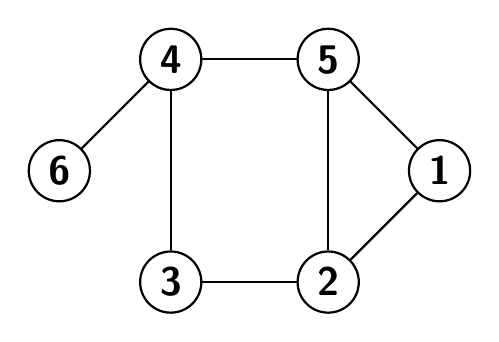
\begin{tikzpicture}[auto, node distance=2cm, every loop/.style={},
                        thick,main node/.style={circle,draw,font=\sffamily\Large\bfseries}]

      \node[main node] (1) {1};
      \node[main node] (2) [below left of=1] {2};
      \node[main node] (3) [left of=2] {3};
      \node[main node] (5) [above left of=1] {5};
      \node[main node] (4) [left of=5] {4};
      \node[main node] (6) [below left of=4] {6};

      \path (1) edge (2);
      \path (1) edge (5);
      \path (5) edge (2);
      \path (5) edge (4);
      \path (4) edge (3);
      \path (3) edge (2);
      \path (4) edge (6);
    \end{tikzpicture}
  \end{center}
\end{ex}

\begin{exercise}\label{ex:graphh}
  Let $ \mathcal{H} = (V, E) $ where $ V = \{A, B, C, D\} $ and $ E = \{ \{A, A\},\allowbreak \{A, B\},\allowbreak \{A, C\} \} $. Draw a diagram of $ \mathcal{H} $.
\end{exercise}

\begin{defn}
  A \textbf{path} $ P $ is an ordered set of nodes, such that each pair $ (\alpha, \beta) $ of consecutive nodes in $ P $ is an element of $ E $.
  A graph is called \textbf{connected} if, for any two nodes, there is a path connecting them.
\end{defn}

\begin{exercise}
  Considering the graph $ \mathcal{G} $ defined in \cref{ex:graphg}, write down three possible paths between 1 and 6.
\end{exercise}

\begin{exercise}
  Within the graph $ \mathcal{H} $ defined in \cref{ex:graphh}, is there a path between $ B $ and $ C $? What about between $ A $ and $ D $?
\end{exercise}

A natural question to ask is whether we can walk through every node of a graph in one go.

\begin{defn}
  A \textbf{Hamiltonian path} is a path on a graph such that every node appears on the path exactly once. If the two endpoints
  of the path are adjacent, then the path is called a \textbf{Hamiltonian cycle}.
\end{defn}

\begin{ex}
  A Hamiltonian path can be found in the graph $ \mathcal{G} $ of \cref{ex:graphg} above:
  \begin{center}
    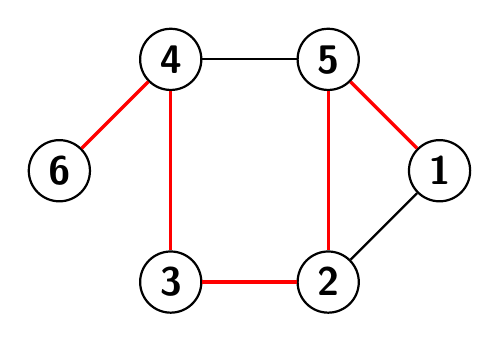
\begin{tikzpicture}[auto, node distance=2cm, every loop/.style={},
                        thick,main node/.style={circle,draw,font=\sffamily\Large\bfseries}]

      \node[main node] (1) {1};
      \node[main node] (2) [below left of=1] {2};
      \node[main node] (3) [left of=2] {3};
      \node[main node] (5) [above left of=1] {5};
      \node[main node] (4) [left of=5] {4};
      \node[main node] (6) [below left of=4] {6};

      \path (1) edge (2);
      \path[color = red, very thick] (1) edge (5);
      \path[color = red, very thick] (5) edge (2);
      \path (5) edge (4);
      \path[color = red, very thick] (4) edge (3);
      \path[color = red, very thick] (3) edge (2);
      \path[color = red, very thick] (4) edge (6);
    \end{tikzpicture}
  \end{center}
\end{ex}

\begin{exercise}
  Find a Hamiltonian cycle on the dodecahedron:\footnote{~From \texttt{https://commons.wikimedia.org/wiki/File:Dodecahedron\_schlegel\_diagram.png}.}
  \begin{center}
    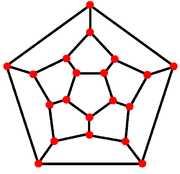
\includegraphics[width=0.3\textwidth]{dodec}
  \end{center}
\end{exercise}

Unfortunately it is difficult to find a general condition to determine whether a graph has a Hamiltonian path, so we turn
our attention to a related concept.

\begin{defn}
  A \textbf{Euler walk} is a path on a graph such that every edge appears on the path exactly once. If the two endpoints
  of the path are adjacent, then the path is called a \textbf{Euler tour}.
\end{defn}

We need a bit of terminology:

\begin{defn}
  The \textbf{degree} of a node is the number of edges connected to it.
\end{defn}

\begin{ex}
  In the graph $ \mathcal{G} $ of \cref{ex:graphg} above, the degree of 6 is 1, the degree of 4 is 3, and the degree of 1 is 2.
\end{ex}

\begin{rem}
  The degree of the node $ X $ in the following graph is defined to be 2.
  \begin{center}
    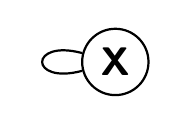
\begin{tikzpicture}[auto, node distance=3cm, every loop/.style={},
                        thick,main node/.style={circle,draw,font=\sffamily\Large\bfseries}]

      \node[main node] (1) {X};

      \path (1) edge[loop left] (1);
    \end{tikzpicture}
  \end{center}
\end{rem}

The following theorem was first stated by Leonhard Euler in 1736.

\begin{thm}[Euler's criteria]
  A \textit{necessary} condition for an Euler walk on a graph is that:
  \begin{itemize}
    \item The graph is connected.
    \item The number of nodes of odd degree must be either zero or two.
  \end{itemize}
\end{thm}

It was proved by Carl Hierholzer that Euler's criteria is in fact \textit{sufficient}: that is, any graph meeting Euler's criteria will have a Euler walk.

\begin{proof}[Proof of Euler's criteria]
  The requirement that the graph must be connected is obvious.

  Except at the end-points of any Euler walk, the number of times that one enters a node must equal the number of times that
  one leaves. Since we cannot use any edge more than once, it follows that the number of edges on each non-terminal
  node must be even. Hence, the only nodes of odd degree can be the end-points and so there are at most two nodes of odd degree.

  Now, suppose that there is exactly one endpoint of odd degree (and suppose that it is the initial endpoint). Then the two endpoints
  are distinct (otherwise both endpoints would be of odd degree), and every time we arrive at the final endpoint we would need to leave
  again (otherwise we would miss out an edge), which is obviously impossible.
\end{proof}

One of the most notable problems in mathematics history is the K\"onigsberg Bridge problem, solved by Euler using the above
result. The problem lead directly to the development of graph theory and topology as mathematical disciplines.

\begin{ex}
  In the city of K\"onigsberg, in Prussia,\footnote{~Now Kaliningrad in Russia.} there were four islands connected by seven bridges as
  in the image.\footnote{~From \texttt{https://en.wikipedia.org/wiki/File:Konigsberg\_bridges.png}.}
  \begin{center}
    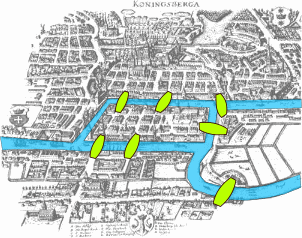
\includegraphics[width=0.4\textwidth]{konig1}
  \end{center}
  The K\"onigsbergians wondered if there was some journey that could cross every bridge exactly once (and obviously avoiding swimming, the use of boats, or of
  other bridges outside the city).

  Euler's main idea was to collapse the relevant topological features into a graph,\footnote{~Image from \texttt{https://en.wikipedia.org/wiki/File:K\%C3\%B6nigsberg\_graph.svg}.} where the nodes represent islands and the edges represent bridges.
  \begin{center}
    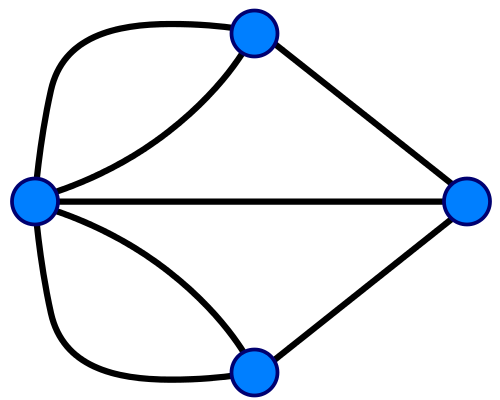
\includegraphics[width=0.3\textwidth]{konig2}
  \end{center}
  Now the problem is simply to find an Euler walk on this graph.
\end{ex}

\begin{exercise}
  Show that there is no Euler walk on the graph of K\"onigsberg.
\end{exercise}

\section{Next Steps}
As well as the material in the level three standards (differentiation, integration, algebra, linear systems, linear programming, path analysis,
trigonometry, and conic sections) it is advantageous for Scholarship students to be aware of mathematics as a broader discipline. In the 2017
paper, for example, the opening question part was on number theory.

As such, I have here a list of books and topics which Scholarship students may wish to look over. I have included the University of Auckland
library call number in brackets.
\begin{itemize}
  \item \textbf{Culture:} \emph{A Mathematician's Lament} by Paul Lockhart [510.71 L81].
  \item \textbf{Proofs:} \emph{How to Think Like a Mathematician} by Kevin Houston [510 H84].
  \item \textbf{Number theory:} \emph{Elementary Number Theory} by Underwood Dudley [512.72 D84].
  \item \textbf{Linear algebra:} \emph{Linear Algebra: A Modern Introduction} by David Poole [512.5 P82].
  \item \textbf{Geometry:} \emph{Geometry: A High School Course} by Serge Lang and Gene Murrow [516 L27].
  \item \textbf{Set theory:} \emph{Naive Set Theory} by Paul Halmos [511.322 H19].
  \item \textbf{Calculus:} \emph{Calculus} by Paul Spivak [515 S76].
\end{itemize}

I must stress that a comprehensive understanding of the content in the above books is \emph{not required}; in most cases, a read of the first three
sections will suffice to obtain an overview of the relevant parts of the subject (not that that precludes interested students from reading further).

\end{document}
